\section{Introduction}

We consider the problem of {\it patrolling} --- i.e. to defend and supervise a given area by one or more agents moving around this and visiting a designated place within the area at a sufficient frequency.~\cite{czyzowicz2011boundary}

Here we consider the following problem. 
One or more agents patrol over an undirected graph with edge lengths by moving on the edges with speed 1 or less. Each point has an {\it allowable visiting interval} and should not be left over that time (conditions of security). Determine if this is possible.

Coene et al.~\cite{coene2011charlemagne} showed several polynomial time algorithms and NP-hardness for some graphs under the assumption that at most one agent who guards each point (uncooperative).
In this research we consider the case of losing constraints of non-cooperation (it may be that there is a point where two or more agents cooperate to guard).


% graph shapes
\section{Shapes of graphs and its complexity}

Since it is NP-hard in the general graph for even a single agent, we picked up Line, Star, Unit as graph shapes.
Line is a graph composed of a series of line segments, Star is a graph whose center point is one end point of all edges and Unit is a complete graph with all edges equal in length.
We assume that the center point of a Star is not a subject to be guarded.
In the patrolling problem, only the distance traveled between the points of the graph is important, so a Unit is equivalent to a Star with all edges equal in length and can be regarded as a special case of Star.


According to Coene et al.~\cite{coene2011charlemagne}, for cases where there is only one agent, polynomial time algorithms are known for Tree with uniform allowable visit intervals or for Line,
and Star with arbitrary allowable visiting intervals is NP-hard.
We aim to give evaluations of the complexity class except in cases where it is already NP-hard for single agent, that is, in the case of (1) Line, (2) Unit, (3) Star with uniform allowable visiting intervals, (4) Tree with uniform allowable visiting intervals.

\begin{figure}[htbp]
  \begin{tabular}{cc}
    \begin{minipage}{0.5\hsize}
      \centering
      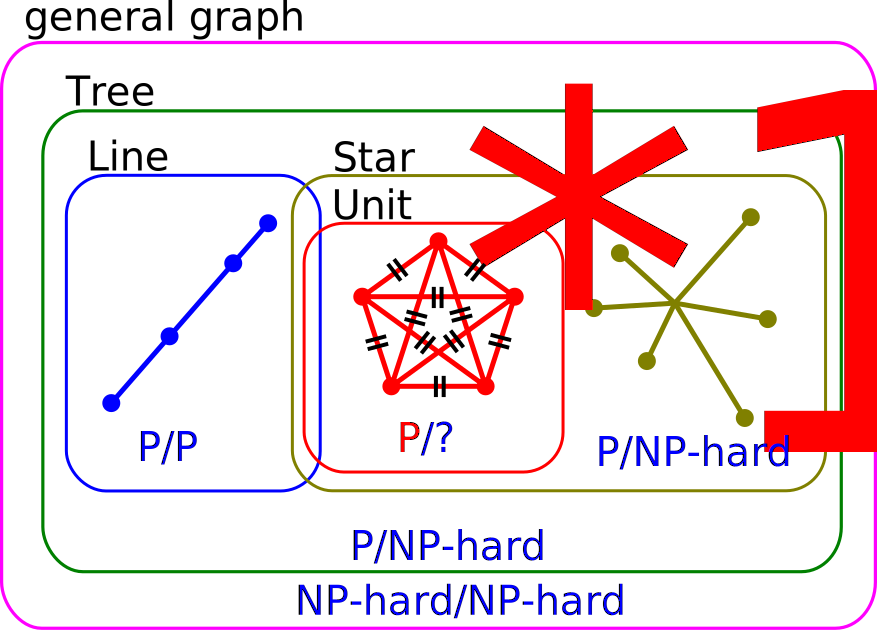
\includegraphics[width=\hsize]{../fig1_adjust.pdf}
    \end{minipage}
    \begin{minipage}{0.5\hsize}
      \centering
      \includegraphics[width=\hsize]{../fig2_adjust.pdf}
    \end{minipage}
  \end{tabular}
  \caption{Shapes of graphs and its complexity.
  The left side of the slash represents the case of uniform allowable visiting intervals, and the right side represents the case of arbitrary allowable visiting intervals}
  \label{fig:shapeandcomplexity}
\end{figure}




\section{Uniform allowable visiting intervals}
For each graph, we first considered the case where the allowable visiting intervals of all points are equal, and we obtained the result that all of them can be calculated in polynomial time.

In the case of Line, it is shown that an optimal strategy for each agent
is a reciprocating motion in some section regardless of other agents' movements.
In the case of Star, it is shown that an optimal strategy is that
each agent resides at a point more than a certain distance from the center point,
and the rest agents move in line at equal intervals of the allowable visiting intervals and visit the remaining points in order.
In this way, it was found that if the cooperation of the agents is unnecessary or when the cooperation method becomes extremely simple due to all equal allowable visiting intervals, it can be easily solved.
In addition, they can also be applied to a problem extended to find a point subset where gains are set for points and the sum of gains is maximized.



\section{Arbitrary allowable visiting intervals}

On the other hand, because it was difficult to evaluate when the allowable visit interval was general in the line segment, Unit, we evaluated the computational complexity class by considering the case of visit time designation as a condition instead of the allowable visit interval defined as the condition of security at each point.
As a result, there are algorithms that greedily determine the motion of the agent in Line
(Figure \ref{fig:shapeandcomplexity}-*2 ),
and in Unit it was shown that it is NP-hard even if there is only one agent by a reduction from the maximum independent set problem
(Figure \ref{fig:shapeandcomplexity}-*1 ).
